\documentclass[12pt,twoside,letterpaper]{book}
%\usepackage{layout}
%\usepackage{makeidx}
\RequirePackage{verbatim}
%\RequirePackage{alltt}
\usepackage{ifpdf}
\usepackage{etoolbox}
\usepackage{multicol}
\usepackage{dsfont}
\usepackage{amsfonts}
\usepackage{amsmath}
\usepackage{array}
%\usepackage{wasysym}
\usepackage{qrcode}

\usepackage{amsmath, amssymb, array}
\usepackage{enumitem}
\usepackage{pgfplots}
\usepackage{graphicx}
\usepackage{lipsum}
\usepackage{stfloats}
\usepackage{multicol}
\setlength{\columnsep}{1cm}

\usepackage{minipage-marginpar}
\setlength{\columnsep}{1cm}
\usepackage{pinlabel} % for pin labels on figure


\newcommand{\boxcolor}{gray!30}
\usepackage{mdframed}
\newenvironment{boxme}{\begin{mdframed}[backgroundcolor=\boxcolor,linewidth=0pt,nobreak=true]}{\end{mdframed}}
\newenvironment{boxthm}{\begin{mdframed}[backgroundcolor=\boxcolor,nobreak=true]}{\end{mdframed}}
\newenvironment{boxdef}{\begin{mdframed}[backgroundcolor=\boxcolor,linewidth=0pt,nobreak=true]}{\end{mdframed}}


% Define a toggle that determines if a large or small print version
% will be printed.
\newtoggle{largePrint}
\toggletrue{largePrint}
\togglefalse{largePrint}

% Define a toggle that determines if solutions are printed. 
% (Not implemented yet)
\newtoggle{solutions}
\toggletrue{solutions}
\togglefalse{solutions}

\usepackage{graphicx}
\usepackage[pass]{geometry}
\usepackage{color}
\usepackage{hyperref}
\hypersetup{
  pdftitle={Recitation Activities for Math 1113, precalculus},
  pdfsubject={precalculus},
  pdfauthor={UGA Mathematics Department},
  pdfkeywords={classroom activities, precalculus},
  anchorcolor = {blue},
  colorlinks = {true},
  runcolor = {black},
  linkcolor = {red},
  urlcolor = {black},
  % pdfpagemode={FullScreen}
}

\usepackage{tikz}
\usepackage{pgf}
\usetikzlibrary{calc,mindmap,backgrounds,arrows,shapes.geometric}
%\usepackage{pstricks}


\pagestyle{myheadings}

%\setlength{\basicoddside}{\oddsidemargin}
%\setlength{\basicevenside}{\evensidemargin}
%\setlength{\basicwidth}{\textwidth}
%\setlength{\basictop}{\topmargin}
%\setlength{\basicheight}{\textheight}


\newcommand{\introduction}[1]{}

\font\tenit=cmti10
\makeatletter

\renewcommand{\@evenfoot}{\tenit University of Georgia Department of
  Mathematics\hfill}
\renewcommand{\@oddfoot}{\tenit \hfill Math 1113 - Precalculus}

\renewcommand{\section}{\@startsection
  {section}
  {1}
  {0em}
  {\baselineskip}
  {-1em}
  {\normalfont\normalsize\bfseries}}

\renewcommand{\subsection}{\@startsection
  {subsection}
  {2}
  {0em}
  {\baselineskip}
  {-1em}
  {\normalfont\normalsize\bfseries}}

\renewcommand{\subsubsection}{\@startsection
  {subsubsection}
  {2}
  {0em}
  {\baselineskip}
  {-2em}
  {\normalfont\normalsize\itshape}}

\makeatother


\newlength{\basicoddside}
\newlength{\basicevenside}
\newlength{\basicwidth}
\newlength{\basictop}
\newlength{\basicheight}

\setlength{\oddsidemargin}{0.15in}
\setlength{\evensidemargin}{0.15in}
\setlength{\textwidth}{6.0in}
\setlength{\topmargin}{-0.5in}
\setlength{\textheight}{9in}
\setlength{\marginparwidth}{52pt}


\newcommand{\activityParams}{
  %\setlength{\hoffset}{0in}
  %\setlength{\oddsidemargin}{-0.5in}
  %\setlength{\evensidemargin}{-0.5in}
  %\setlength{\textwidth}{7.5in}
  \setlength{\topmargin}{-0.5in}
  \setlength{\textheight}{9in}
}

\newcommand{\textParams}{
  \setlength{\oddsidemargin}{\basicoddside}
  \setlength{\evensidemargin}{\basicevenside}
  \setlength{\textwidth}{\basicwidth}
  \setlength{\topmargin}{\basictop}
  \setlength{\textheight}{\basicheight}
}



\newcommand{\sideNote}[1]{\marginpar{\tenit \raggedright #1}}
\newcommand{\doNotPrint}[1]{}


\newtheorem{lemma}{Lemma}[subsection]
\newtheorem{theorem}{Theorem}[subsection]



\newcounter{activity}
\setcounter{activity}{1}

\newcommand{\actTitle}[1]{
  \cleardoublepage
  \activityParams
  \stepcounter{activity}
  \markboth
  {Name: \hspace*{2.5in} \hfil  In-Class Activity: \theactivity}
  {Name: \hspace*{2.5in} \hfil  In-Class Activity: \theactivity}
  \stepcounter{section}
  \addcontentsline{toc}{section}{
    \protect\numberline{\thesection}{#1}}
}

\newcounter{hw}
\setcounter{hw}{0}
\newcommand{\hwTitle}[1]{
  \cleardoublepage
  \activityParams
  \stepcounter{hw}
  \markboth
  {Name: \hspace*{2.5in} \hfil  Home Work: \thehw}
  {Name: \hspace*{2.5in} \hfil  Home Work: \thehw}
  \stepcounter{subsubsection}
  \addcontentsline{toc}{subsubsection}{
    \protect\numberline{\thesubsubsection}{#1}}
}

\newcommand{\preClass}[1]{
  \cleardoublepage
  \activityParams
  \markboth
  {Name: \hspace*{2in} \hfil Preclass Work - Finish Before Class Begins \hfil}
  {Name: \hspace*{2in} \hfil Preclass Work - Finish Before Class Begins \hfil}
  \stepcounter{subsubsection}
  \addcontentsline{toc}{subsubsection}{
    \protect\numberline{\thesubsubsection}{#1}}
}

\newcommand{\postClass}{

  \cleardoublepage
  \activityParams
  \markboth
  {Name: \hspace*{2in} \hfil Postclass Work - Finish After Class \hfil}
  {Name: \hspace*{2in} \hfil Postclass Work - Finish After Class \hfil}
%  \stepcounter{subsubsection}
%  \addcontentsline{toc}{subsubsection}{
%    \protect\numberline{\thesubsubsection}{#1}}
}


\newcounter{quiz}
\setcounter{quiz}{1}
\newcommand{\qzTitle}[1]{
  \cleardoublepage
  \activityParams
  \stepcounter{quiz}
  \markboth
  {Name: \hspace*{2.5in} \hfil  #1 Quiz: \thequiz ~~~ }
  {Name: \hspace*{2.5in} \hfil  #1 Quiz: \thequiz ~~~ }
  \stepcounter{subsubsection}
  \addcontentsline{toc}{subsubsection}{
    \protect\numberline{\thesubsubsection}{#1}}
}

\newcounter{properties}
\setcounter{properties}{1}
\newcommand{\propertiesTitle}[1]{
  \cleardoublepage
  \activityParams
  \stepcounter{properties}
  \markboth
  {Name: \hspace*{2.5in} \hfil  #1 (Properties: \theproperties) ~ }
  {Name: \hspace*{2.5in} \hfil  #1 (Properties: \theproperties) ~ }
  \stepcounter{subsubsection}
  \addcontentsline{toc}{subsubsection}{
    \protect\numberline{\thesubsubsection}{#1}}
}


\newcommand{\stateSummary}{\item State and summarize two ideas from today's
  class. 
  \vfill 
  \centerline{\textit{(Over)}}
  \clearpage }


\newcommand{\addTOC}[1]{
  \stepcounter{section}
  \addcontentsline{toc}{section}{
    \protect\numberline{\thesection}{#1}}
  }



\newenvironment{problem}
{\begin{list}
{\arabic{enumi}.}
{\usecounter{enumi}
\setlength{\rightmargin}{0pt}
%\setlength{\rightmargin}{-72pt}
\setlength{\parsep}{0em}
\setlength{\listparindent}{0pt}
}}
{\end{list}}

\newenvironment{subproblem}
{\begin{list}
{(\alph{enumii})}
{\usecounter{enumii}
\setlength{\rightmargin}{0pt}
\setlength{\parsep}{1em}
\setlength{\listparindent}{0pt}
}}
{\end{list}}

\newenvironment{subsubproblem}
{\begin{list}
{(\roman{enumiii})}
{\usecounter{enumiii}
\setlength{\rightmargin}{0pt}
\setlength{\parsep}{1em}
\setlength{\listparindent}{0pt}
}}
{\end{list}}

\newenvironment{multiEqn}
{\begin{eqnarray*} 
 \begin{array}{rclclclcl}}
{\end{array}
 \end{eqnarray*}}


\setcounter{activity}{0}


% %%%%%%%%%%%%%%%%%%%%%%%%%%%%%%%%%%%%%%%%%%%%%%%%%%%%%%%%%%%%%%%%%%%%%%%
% List of definitions that are used in the different pages for the
% notes

% %%%%%%%%%%%%%%%%%%%%%%%%%%%%%%%%%%%%%%%%%%%%%%%%%%%%%%%%%%%%%%%%%%%%%%%
% Basic latex commands used throughout the notes.

\newcommand{\videoLink}[2]{%

  \noindent
  Watch the Pre-Class videos for #1 and answer the following
  questions. Remember that in your written work you are graded on the
  correctness of your supporting work and not just your final
  answer. Always give an exact answer unless you are explicitly told
  to round; calculator approximations will not receive full credit.

  \qrcode[height=2.0cm,hyperlink,tight]{#2}

  \bigskip

}

% Basic mathematical definitions used throughout the notes

\newcommand{\change}[1]{\triangle #1}
\newcommand{\fortyFive}{\frac{\sqrt{2}}{2}}
\newcommand{\imag}{j}
\newcommand{\half}{\mbox{$\frac{1}{2}$}}
\newcommand{\deltat}{\mbox{$\triangle t$}}
\newcommand{\deltax}{\mbox{$\triangle x$}}
\newcommand{\deltay}{\mbox{$\triangle y$}}

\newcommand{\deriv}[2]{\frac{d}{d#2}#1}
\newcommand{\derivTwo}[2]{\frac{d^2}{d#2^2}#1}

\newcommand{\lp}{\left(}
\newcommand{\rp}{\right)}


% %%%%%%%%%%%%%%%%%%%%%%%%%%%%%%%%%%%%%%%%%%%%%%%%%%%%%%%%%%%%%%%%%%%%%%
% trigonometry definitions
\newcommand{\trigTriangle}[5]{%
	\begin{tikzpicture}[scale=2.5]
	\draw (0,0) -- (2,0) -- (2,1) -- (0,0);
	\draw (1.9,0) -- (1.9,0.1) -- (2,0.1);
	\draw (0.3,0) arc(0:40:0.2);
	\draw (0.5,0.1) node { #1 };
	\draw (1.8,0.7) node { #2 };
	\draw (1,-0.1) node { #3 };
	\draw (1,0.6) node { #4 };
	\draw (2,0.8) arc(270:210:0.2);
	\draw (2.1,0.5) node { #5 };
	\end{tikzpicture}
}


% %%%%%%%%%%%%%%%%%%%%%%%%%%%%%%%%%%%%%%%%%%%%%%%%%%%%%%%%%%%%%%%%%%%%%%
% Basic linear algebra commands

\newcommand{\arrayTwo}[4]{
  \left[
  \begin{array}{rr}
    #1 & #2 \\
    #3 & #4
  \end{array}
  \right]
}

\newcommand{\vecTwo}[2]{
  \left[
  \begin{array}{r}
    #1 \\  #2
  \end{array}
  \right]
}

\newcommand{\vecFour}[4]{
  \left[
  \begin{array}{r}
    #1 \\  #2 \\ #3 \\ #4
  \end{array}
  \right]
}


\newcommand{\stateTwo}[2]{
  \begin{array}{rr}
    \mbox{\fontsize{6}{6}\selectfont $#1$} \\  \mbox{\fontsize{6}{6}\selectfont $#2$}
  \end{array}
}


\newcommand{\arrayThree}[9]{
  \left[
    \begin{array}{rrr}
      #1 & #2 & #3 \\
      #4 & #5 & #6 \\
      #7 & #8 & #9
    \end{array}
  \right]
}

\newcommand{\startRowOps}{
  \left[
    \begin{array}{rrr|r}
}

\newcommand{\oneRowOps}[4] {
      #1 & #2 & #3 & #4 \\
}

\newcommand{\stopRowOps}{
    \end{array}
  \right]
}


\newcommand{\vecThree}[3]{
  \left[
  \begin{array}{r}
    #1 \\  #2 \\ #3
  \end{array}
  \right]
}


\newcommand{\stateThree}[3]{
  \begin{array}{r}
    \mbox{\fontsize{6}{6}\selectfont $#1$} \\  
    \mbox{\fontsize{6}{6}\selectfont $#2$} \\ 
    \mbox{\fontsize{6}{6}\selectfont $#3$}
  \end{array}
}





\newcommand{\detTwo}[4]{
  \left|
  \begin{array}{rr}
    #1 & #2 \\
    #3 & #4
  \end{array}
  \right|
}



\newcommand{\detThree}[9]{
  \left|
    \begin{array}{rrr}
      #1 & #2 & #3 \\
      #4 & #5 & #6 \\
      #7 & #8 & #9
    \end{array}
  \right|
}




\newcommand{\startRowFour}{
  \left[
    \begin{array}{rrrr}
}

\newcommand{\oneRowFour}[4] {
      #1 & #2 & #3 & #4 \\
}




\newcommand{\startRowOpsTwo}{
  \left[
    \begin{array}{rr|rr}
}

\newcommand{\oneRowOpsTwo}[4] {
      #1 & #2 & #3 & #4 \\
}


\newcommand{\startRowOpsThree}{
  \left[
    \begin{array}{rrr|rrr}
}

\newcommand{\oneRowOpsThree}[6] {
      #1 & #2 & #3 & #4 & #5 & #6 \\
}





%%% Local Variables: 
%%% mode: latex
%%% TeX-master: t
%%% End: 


\begin{document}



\actTitle{Worksheet 4.3}



\noindent \textbf{Instructions:}  Work together in groups of  3 or 4 to complete the following problems.\\


\begin{enumerate}

\item Find the exact values of the six trigonometric functions of $\theta$ and $\alpha$
\begin{enumerate}
\item Use the following triangle.\\

\newcommand{\trigTriangle}[5]{%
	\begin{tikzpicture}[scale=2.5]
	\draw (0,0) -- (2,0) -- (2,1) -- (0,0);
	\draw (1.9,0) -- (1.9,0.1) -- (2,0.1);
	\draw (0.3,0) arc(0:40:0.2);
	\draw (0.5,0.1) node { #1 };
	\draw (1.8,0.7) node { #2 };
	\draw (1,-0.1) node { #3 };
	\draw (1,0.6) node { #4 };
	\draw (2,0.8) arc(270:210:0.2);
	\draw (2.1,0.5) node { #5 };
	\end{tikzpicture}
}

	\trigTriangle{$\theta$}{$\alpha$}{8}{10}{6}

\vfill
\item Use the following triangle.\\
\trigTriangle{$\theta$}{$\alpha$}{15}{ }{8}
\vfill
\end{enumerate}

\newpage 

\item Use the isosceles right triangle and the 30/60/90 triangle to complete the table.

\begin{table}[h]
\begin{tabular}{|l|l|l|l|l|l|l|}
\hline
\textbf{$\theta$}        & \textbf{$\sin(\theta)$} & \textbf{$\cos(\theta)$} & \textbf{$\tan(\theta)$} & \textbf{$\csc(\theta)$} & \textbf{$\sec(\theta)$} & \textbf{$\cot(\theta)$} \\ \hline
30$^\circ=\frac{\pi}{6}$ &                         &                         &                         &                         &                         &                         \\ \hline
45$^\circ=\frac{\pi}{4}$ &                         &                         &                         &                         &                         &                         \\ \hline
60$^\circ=\frac{\pi}{3}$ &                         &                         &                         &                         &                         &                         \\ \hline
\end{tabular}
\end{table}

\begin{tikzpicture}[y=5cm, x=5cm,font=\sffamily]
  \draw[thick,black] (0,0) -- (1,0) -- (1,1) -- cycle;
  \draw[very thin,black] (0.8,0.0) -- (0.8,0.2) -- (1,0.2);
  \draw[thin,black] (0.2,0) arc (0:45:0.2);
  \node[black,anchor=north] at (0.5,0) {1};
  \node[black,anchor=west] at (1,0.5) {1};
  \node[black,anchor=south east] at (45:0.7) {$\sqrt{2}$};
  \node[black,anchor=south west] at (12.5:0.2) {$45^\circ$};

  \draw[thin,black] (45:1.25) arc (225:270:0.17);
  \node[black,anchor=west,xshift={8pt}] at (45:1.1) {$45^\circ$};
\end{tikzpicture}

\begin{tikzpicture}[y=5cm, x=5cm,font=\sffamily]
  \draw[thick,black] (0,0) -- (1,0) -- (60:2) -- cycle;
  \draw[thick,black,dashed] (1,0) -- (2,0) -- (60:2);
  \draw[very thin,black] (0.8,0.0) -- (0.8,0.2) -- (1,0.2);
  \draw[thin,black] (0.2,0) arc (0:60:0.2);
  \node[black,anchor=north] at (0.5,0) {1};
  \node[black,anchor=west] at (1,0.8) {$\sqrt{3}$};
  \node[black,anchor=south east] at (60:1) {$2$};
  \node[black,anchor=south west] at (12.5:0.2) {$60^\circ$};
  \draw[thin,black] (60:1.8) arc (240:270:0.2);
  \node[black,anchor=west] at (60:1.65) {$30^\circ$};
\end{tikzpicture}

\vfill

%\item
%\begin{enumerate}
%\item Evaluate $\sin(60^\circ)$.\\[0.2in]
%\item Evaluate $\sin(30^\circ)+\sin(30^\circ)$.\\[0.2in]
%\item Are the values in parts $(a)$ and $(b)$ the same?
%\end{enumerate}

\newpage




\item For each problem below determine the values of the missing quantities. All angles are in radians, and your answers for angles should be in radians. (The triangles are not drawn to scale.)
\begin{enumerate}
\item \newcommand{\trigTriangle}[5]{%
	\begin{tikzpicture}[scale=2.5]
	\draw (0,0) -- (2,0) -- (2,1) -- (0,0);
	\draw (1.9,0) -- (1.9,0.1) -- (2,0.1);
	\draw (0.3,0) arc(0:40:0.2);
	\draw (0.5,0.1) node { #1 };
	\draw (1.8,0.7) node { #2 };
	\draw (1,-0.1) node { #3 };
	\draw (1,0.6) node { #4 };
	\draw (2,0.8) arc(270:210:0.2);
	\draw (2.1,0.5) node { #5 };
	\end{tikzpicture}
}



\trigTriangle{$\pi/4$}{$\alpha$}{a}{4}{b}
	
	\framebox[0.3\textwidth][l]{
		\begin{tabular}{lc}
			$a$ & $=$ \\ [15pt]
			$b$ & $=$ \\ [15pt]
			$\alpha$ & $=$ \\
		\end{tabular}
	}
	\vfill

\item \trigTriangle{$\pi/6$}{$\psi$}{2}{h}{b}
	
	\framebox[0.3\textwidth][l]{
		\begin{tabular}{lc}
			$b$ & $=$ \\ [15pt]
			$h$ & $=$ \\ [15pt]
			$\psi$ & $=$ \\
		\end{tabular}
	}
	\vfill

\end{enumerate}
\newpage

\item If a 15 ft ladder is leaning against a wall at an angle of $62^\circ$ with the ground, how high up the will will the ladder reach?  Round to the nearest tenth of a foot.\vfill

\item A 30 ft boat ramp makes a $7^\circ$ angle with the water.  What is the height of the ramp above the water at the ramp's highest point?  Round to the nearest tenth of a foot.\vfill

\item At a tree farm, palm trees are harvested once they reach a height of 20 feet.  Suppose a farm worker determine's that the distance along the ground from her position to the base of a palm tree is 22 feet.  She then uses an instrument called a clinometer held at her eye level of 6 feet to measure the angle of elevation tot he top of the tree as $30.2^\circ$.  Is the tree tall enough to harvest?\vfill
%\newpage
%
%\item The following is the unit circle.  \\
%\includegraphics[scale=.7]{unit_circle}
%\begin{enumerate}
%\item Use the first quadrant to verify your answers in the table in Question 2.\\
%\item Determine the radius of this circle.\\
%
%\end{enumerate}
\end{enumerate}




\end{document}
